
% ---------- Figure snippets (paste into your article) ----------

\begin{figure}[htbp]
\centering
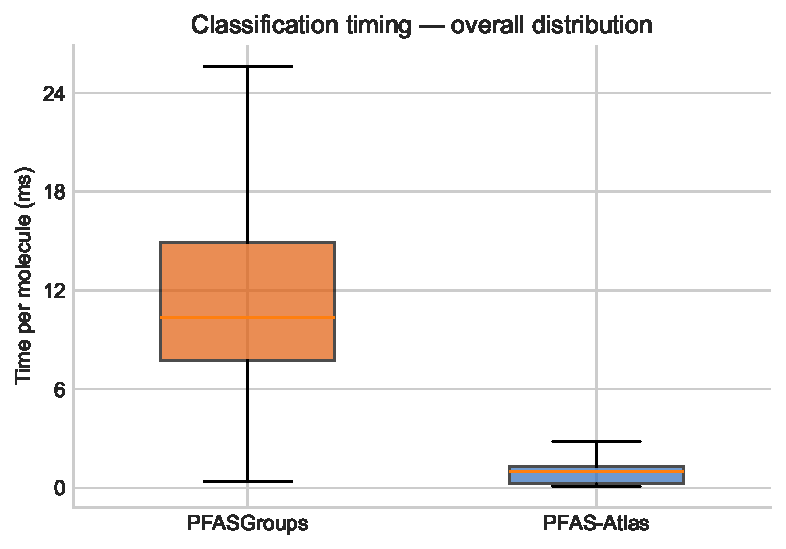
\includegraphics[width=0.7\textwidth]{imgs/clinventory_timing_box.pdf}
\caption{Box plots of per-molecule classification time (ms) for HalogenGroups
  and PFAS-Atlas on the C\&L inventory.  Outliers are omitted.}
\label{fig:clinventory_timing_box}
\end{figure}

\begin{figure}[htbp]
\centering
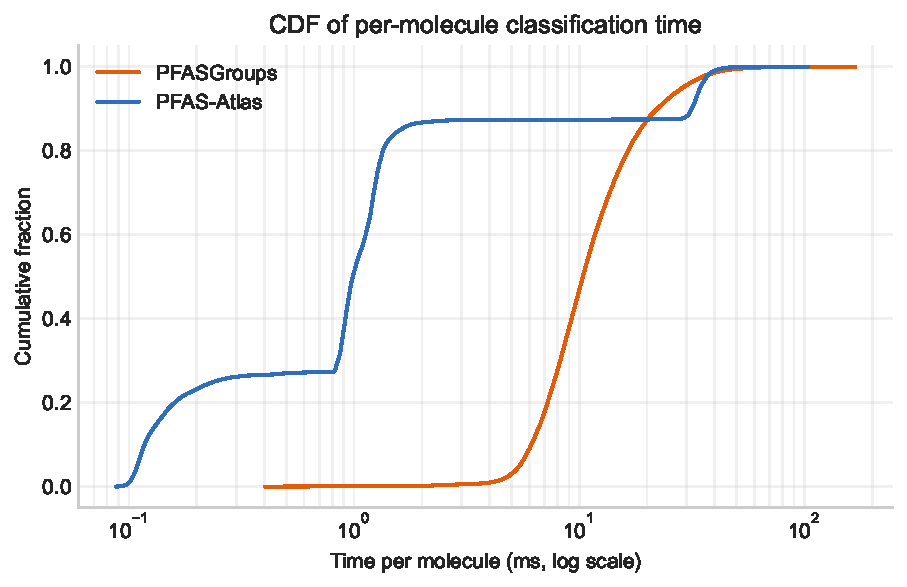
\includegraphics[width=0.85\textwidth]{imgs/clinventory_timing_cdf.pdf}
\caption{Empirical CDF of per-molecule classification time (log scale).}
\label{fig:clinventory_timing_cdf}
\end{figure}

\begin{figure}[htbp]
\centering
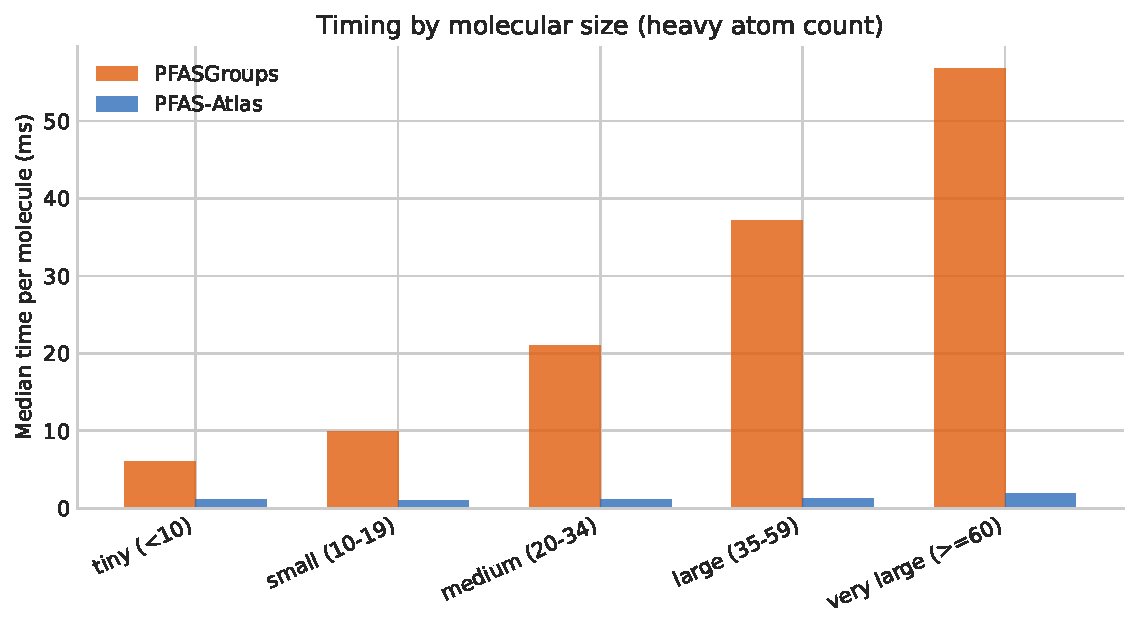
\includegraphics[width=0.9\textwidth]{imgs/clinventory_timing_by_bracket.pdf}
\caption{Median classification time by heavy-atom-count bracket.}
\label{fig:clinventory_timing_bracket}
\end{figure}

\begin{figure}[htbp]
\centering
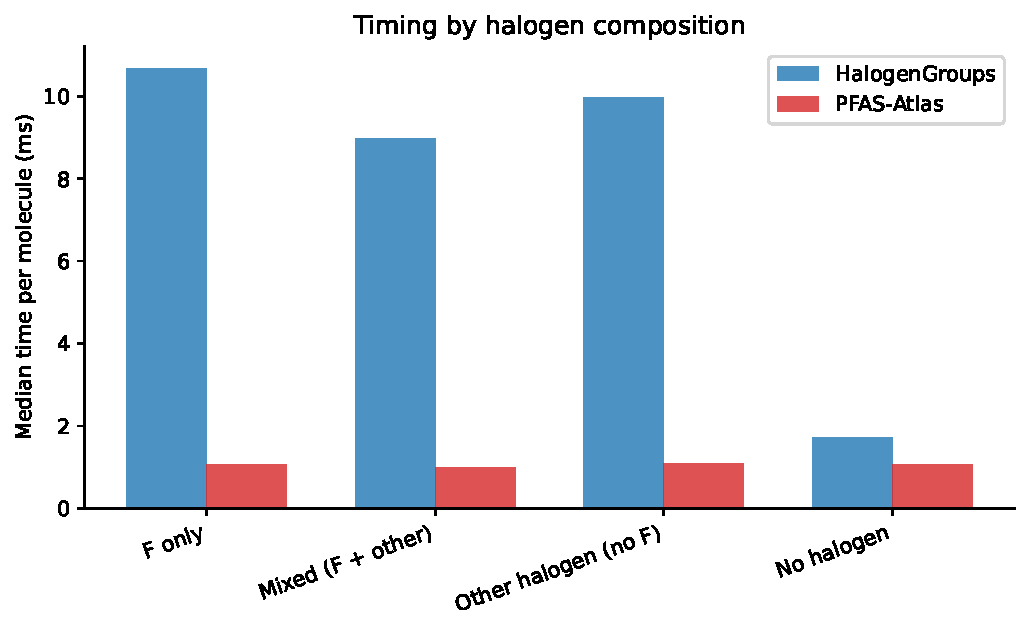
\includegraphics[width=0.85\textwidth]{imgs/clinventory_timing_by_halogen.pdf}
\caption{Median classification time by halogen-composition class.}
\label{fig:clinventory_timing_halogen}
\end{figure}

\begin{figure}[htbp]
\centering
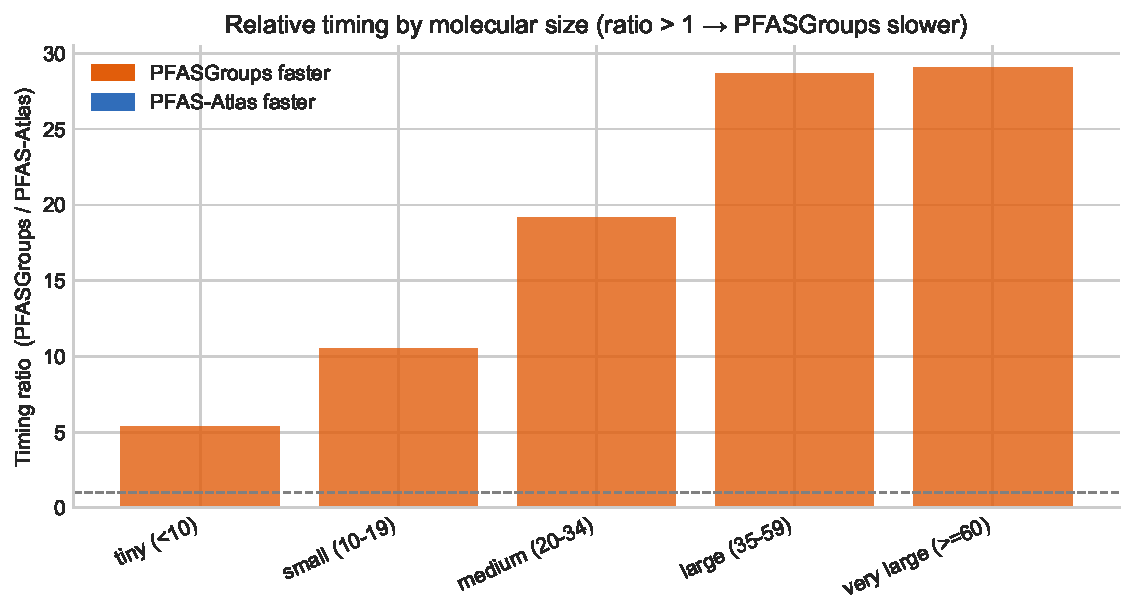
\includegraphics[width=0.9\textwidth]{imgs/clinventory_timing_ratio_by_bracket.pdf}
\caption{Ratio of HalogenGroups to PFAS-Atlas median timing per bracket.
  Values above 1 indicate HalogenGroups is slower; below 1 it is faster.}
\label{fig:clinventory_timing_ratio}
\end{figure}

\begin{figure}[htbp]
\centering
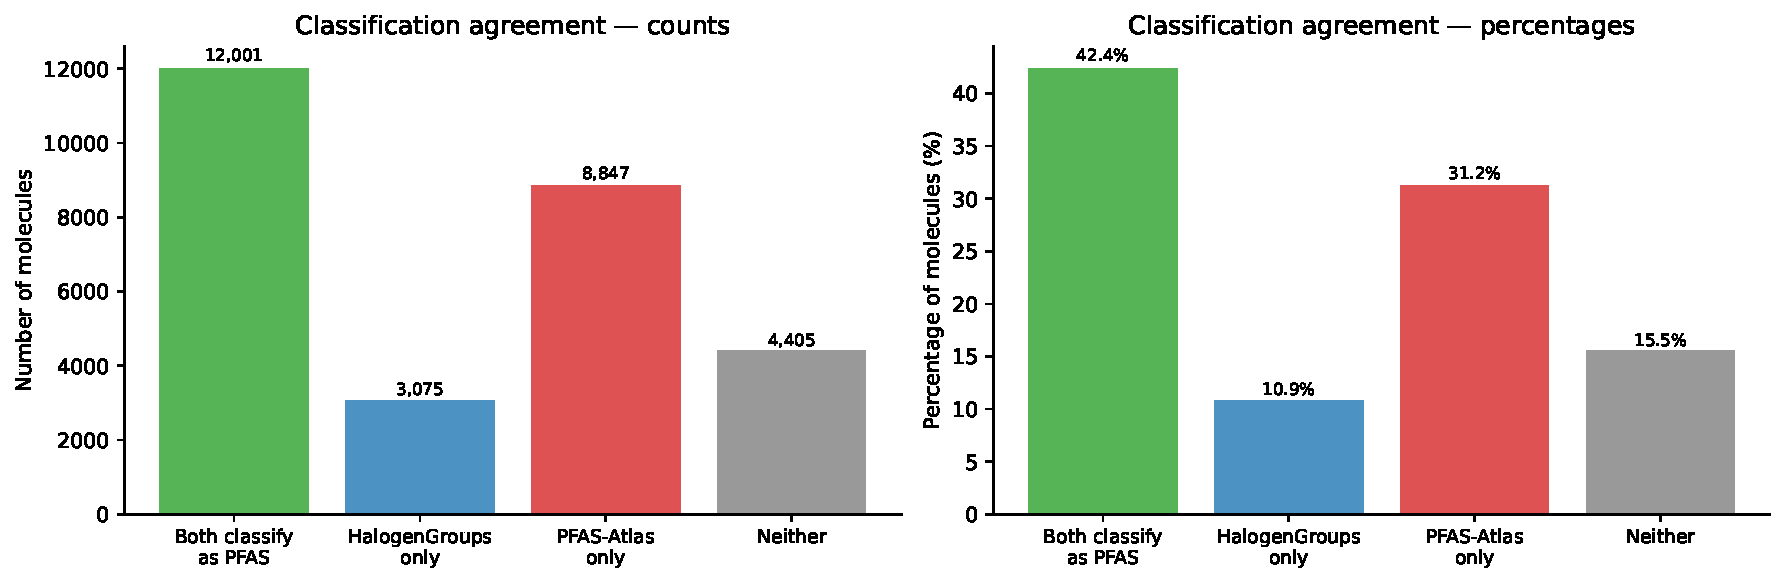
\includegraphics[width=0.9\textwidth]{imgs/clinventory_classification_agreement.pdf}
\caption{Classification agreement between HalogenGroups (F-group detection)
  and PFAS-Atlas (PFAS classification) across the common molecule set.}
\label{fig:clinventory_agreement}
\end{figure}

\begin{figure}[htbp]
\centering
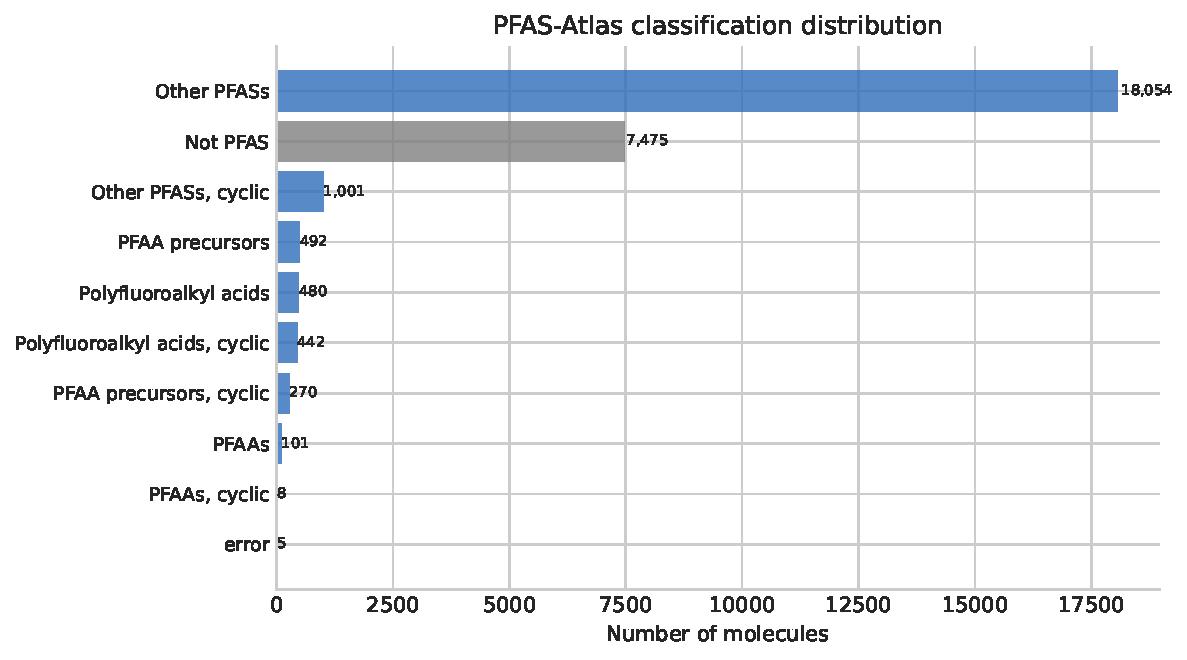
\includegraphics[width=0.75\textwidth]{imgs/clinventory_atlas_class_distribution.pdf}
\caption{Distribution of PFAS-Atlas primary classifications.}
\label{fig:clinventory_atlas_dist}
\end{figure}

\begin{figure}[htbp]
\centering
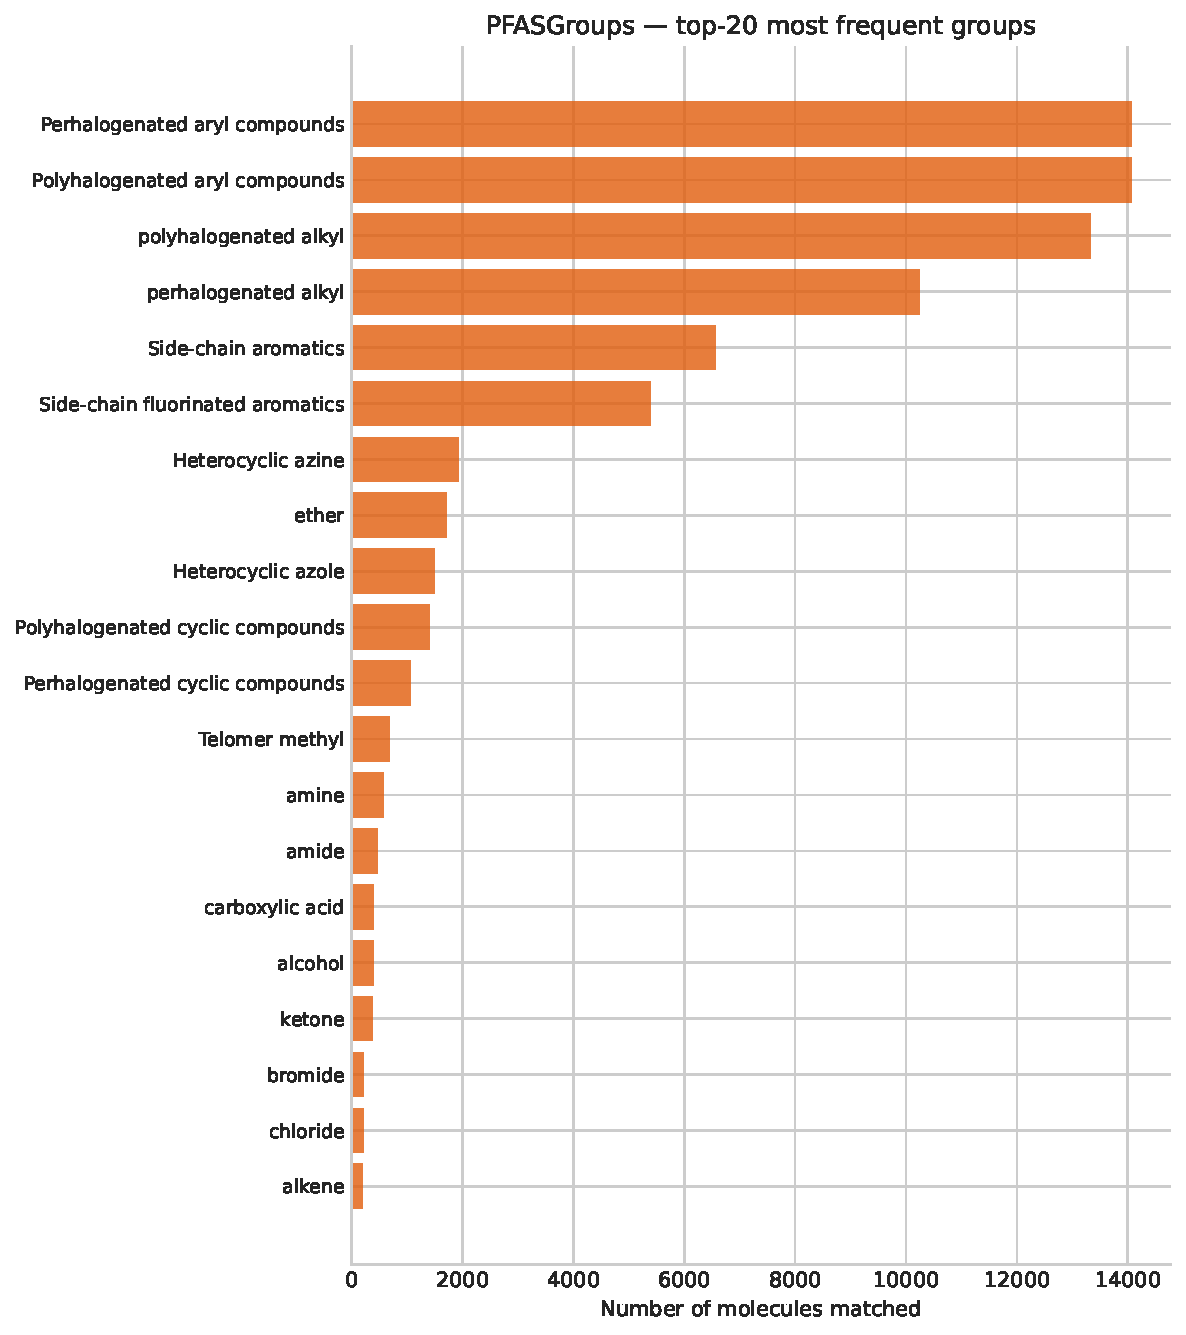
\includegraphics[width=0.75\textwidth]{imgs/clinventory_hg_top_groups.pdf}
\caption{Top-20 most frequently detected HalogenGroups functional groups.}
\label{fig:clinventory_hg_groups}
\end{figure}
